%% !TeX root = main.tex

\chapter{Orthogonal Frequency-Division Multiplexing (OFDM) Project}
\glsresetall
\label{chapter:ofdm}

\section{Introduction}

In this project, you will learn the very basic idea behind an OFDM system, and implement a simple OFDM receiver in programmable logic.  The project is divided into three parts. The first provides an OFDM transmitter and receiver in Simulink. This gives you insight into the ideas behind OFDM. In the second part, you develop a basic OFDM receiver using HLS. The receiver consists of a \gls{fft} module and a QPSK symbol decoder. The final part is to integrate the receiver onto the  Zedboard using Xillybus to transmit data to the OFDM receiver, and receive the decoded data back from your hardware implementation in the programmable logic. You should use Gplot to show the transmitted and received data as you have done in previous projects.

\section{Part I: Simulink}

We provided a Simulink file with an OFDM transmitter, simulated channel, and receiver design. The goal of this part of the project is to gain an initial understanding of how a very simple OFDM system works. Furthermore, you will use the Simulink file to extract data as a testbench for Parts II and III. In this part, we walk you through a series of steps to familiarize you with Simulink and OFDM. This part is optional in the sense you do not have to turn anything. Though you will need to have at least a decent understand of the Simulink in order to complete the assignments from the next two parts of this project. 

Because the HDL-compatible \gls{fft} block inherently bit-reverses, there are two different Simulink models.
\begin{itemize}
\item Version a: No bit reversal in TX, bit reversal in both HDL and behavioral/algorithmic RX, and thus would provide suitable incoming data for a non-bit-reversing Vivado \gls{fft} receiver.
\item Version b: Bit reversal in TX and in both RX  thus be used with a bit-reversing Vivado \gls{fft} receiver.
\end{itemize}

The simple OFDM transmitter encodes 2-bit data symbol (either values of 0 through 3 or random) onto a digital QPSK modulation pattern. 1024 of these symbols go through a 1024-point blockwise I\gls{fft} and are then converted to floating point and sent over a simulated AWGN channel. Two receiver architectures are provided in parallel: HDL-optimized \gls{fft} and block \gls{fft}. You can synthesize the HDL \gls{fft} into Verilog and then run that through Vivado (not HLS) to obtain FPGA resource use estimates.

\begin{figure}
\centering
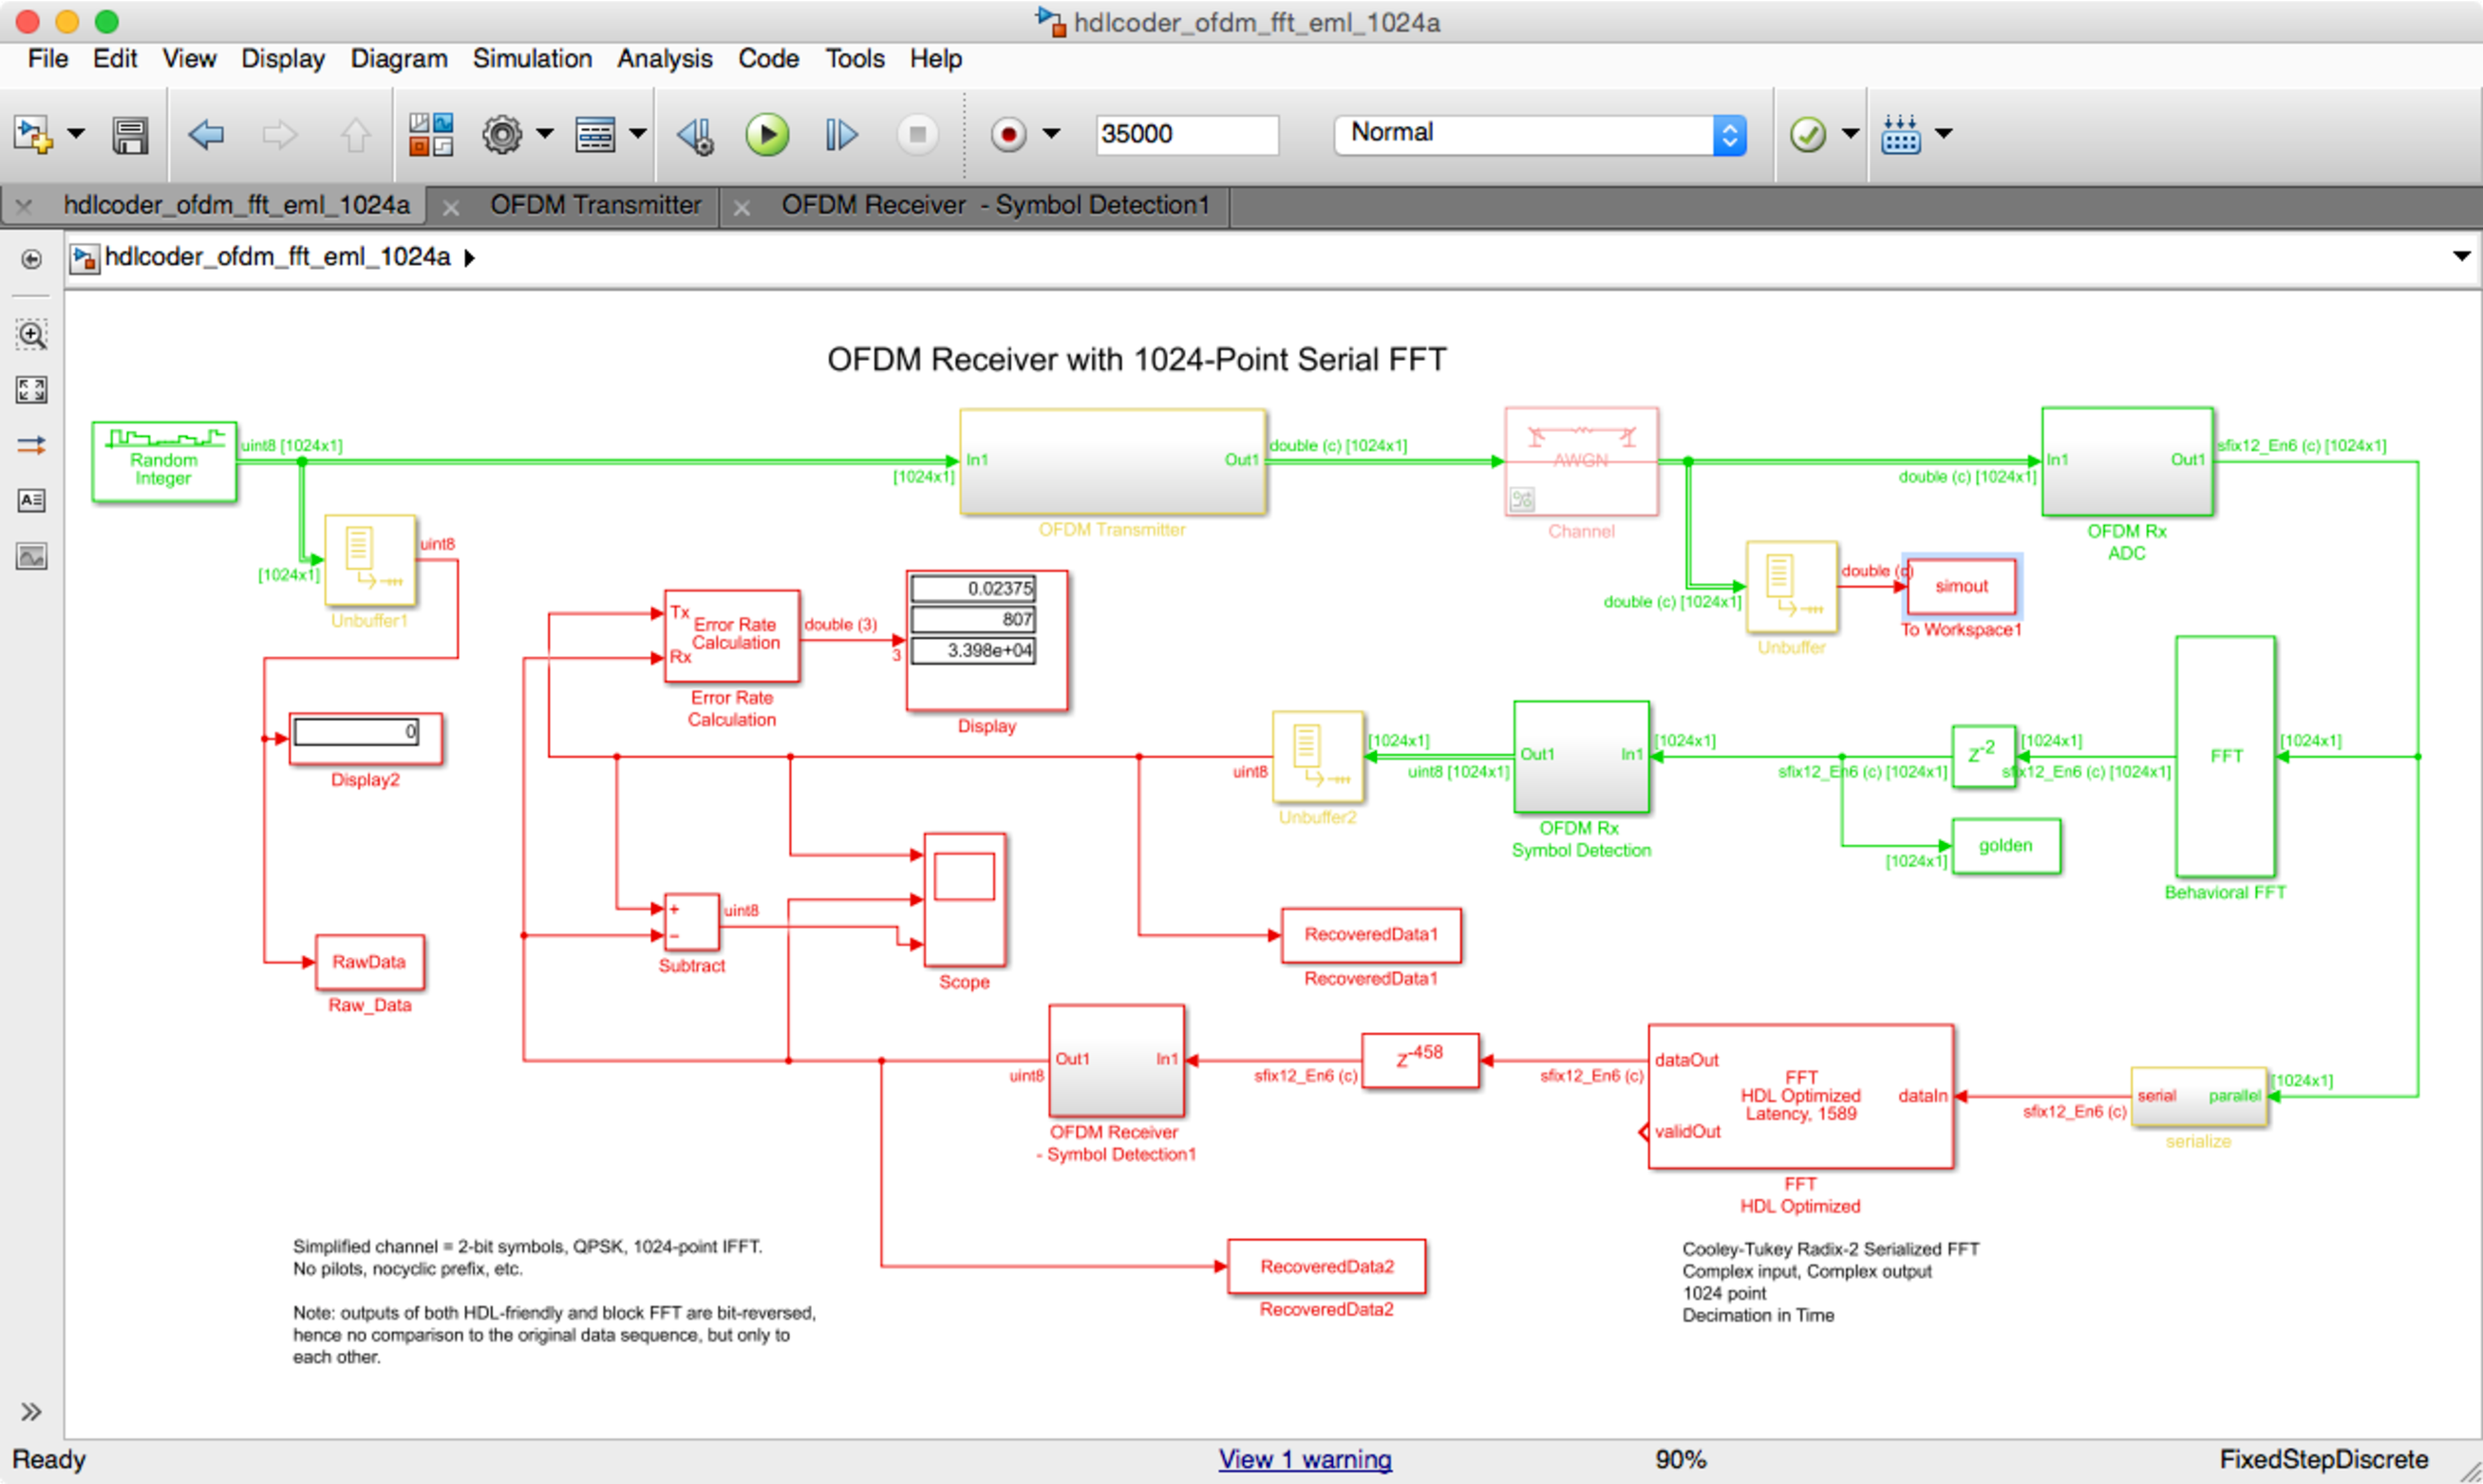
\includegraphics[width=5.5in]{images/ofdm_1024a}
\caption{Simulink test bench for a simple OFDM transceiver. This is found in the Simulink file \texttt{hdlcoder\_ofdm\_fft\_eml\_1024b.slx}.}
\label{fig:ofdm_1024a}
\end{figure}

Figure \ref{fig:ofdm_1024a} shows the top level of the provided \texttt{hdlcoder\_ofdm\_fft\_eml\_1024b.slx} file. The 2-bit/symbol data source is at upper left, the transmitter (QPSK + I\gls{fft}) is top center, then the AWGN simulated channel and the OFDM A/D converter. We do everything except the channel math in fixed point, since we are trying to build real hardware. The channel, is not synthesizable into Verilog or hardware, is kept in floating point, in deference to the computational limits of Matlab, which needs to add Gaussian-distributed random numbers to what we transmit into the channel.

Run the simulation and note the resulting bit error rate and scope traces. Note that the transmitter input and the receiver output have been manually time-aligned for you. In a real system this function will be handled by the synchronization correlators (matched filters), such as those we studied in an earlier projects (e.g., Chapter \ref{chapter:phase_detector}). The z-2 block delays the \texttt{Behavioral\gls{fft}} output by two frames = 2048 sample times, to compensate for the 1589 delays through the HDL Optimized \gls{fft}, the 458 delays after it, and one delay for serializer in front of it. You can see from the scope that the two have been aligned by the external delays.

\begin{figure}
\centering
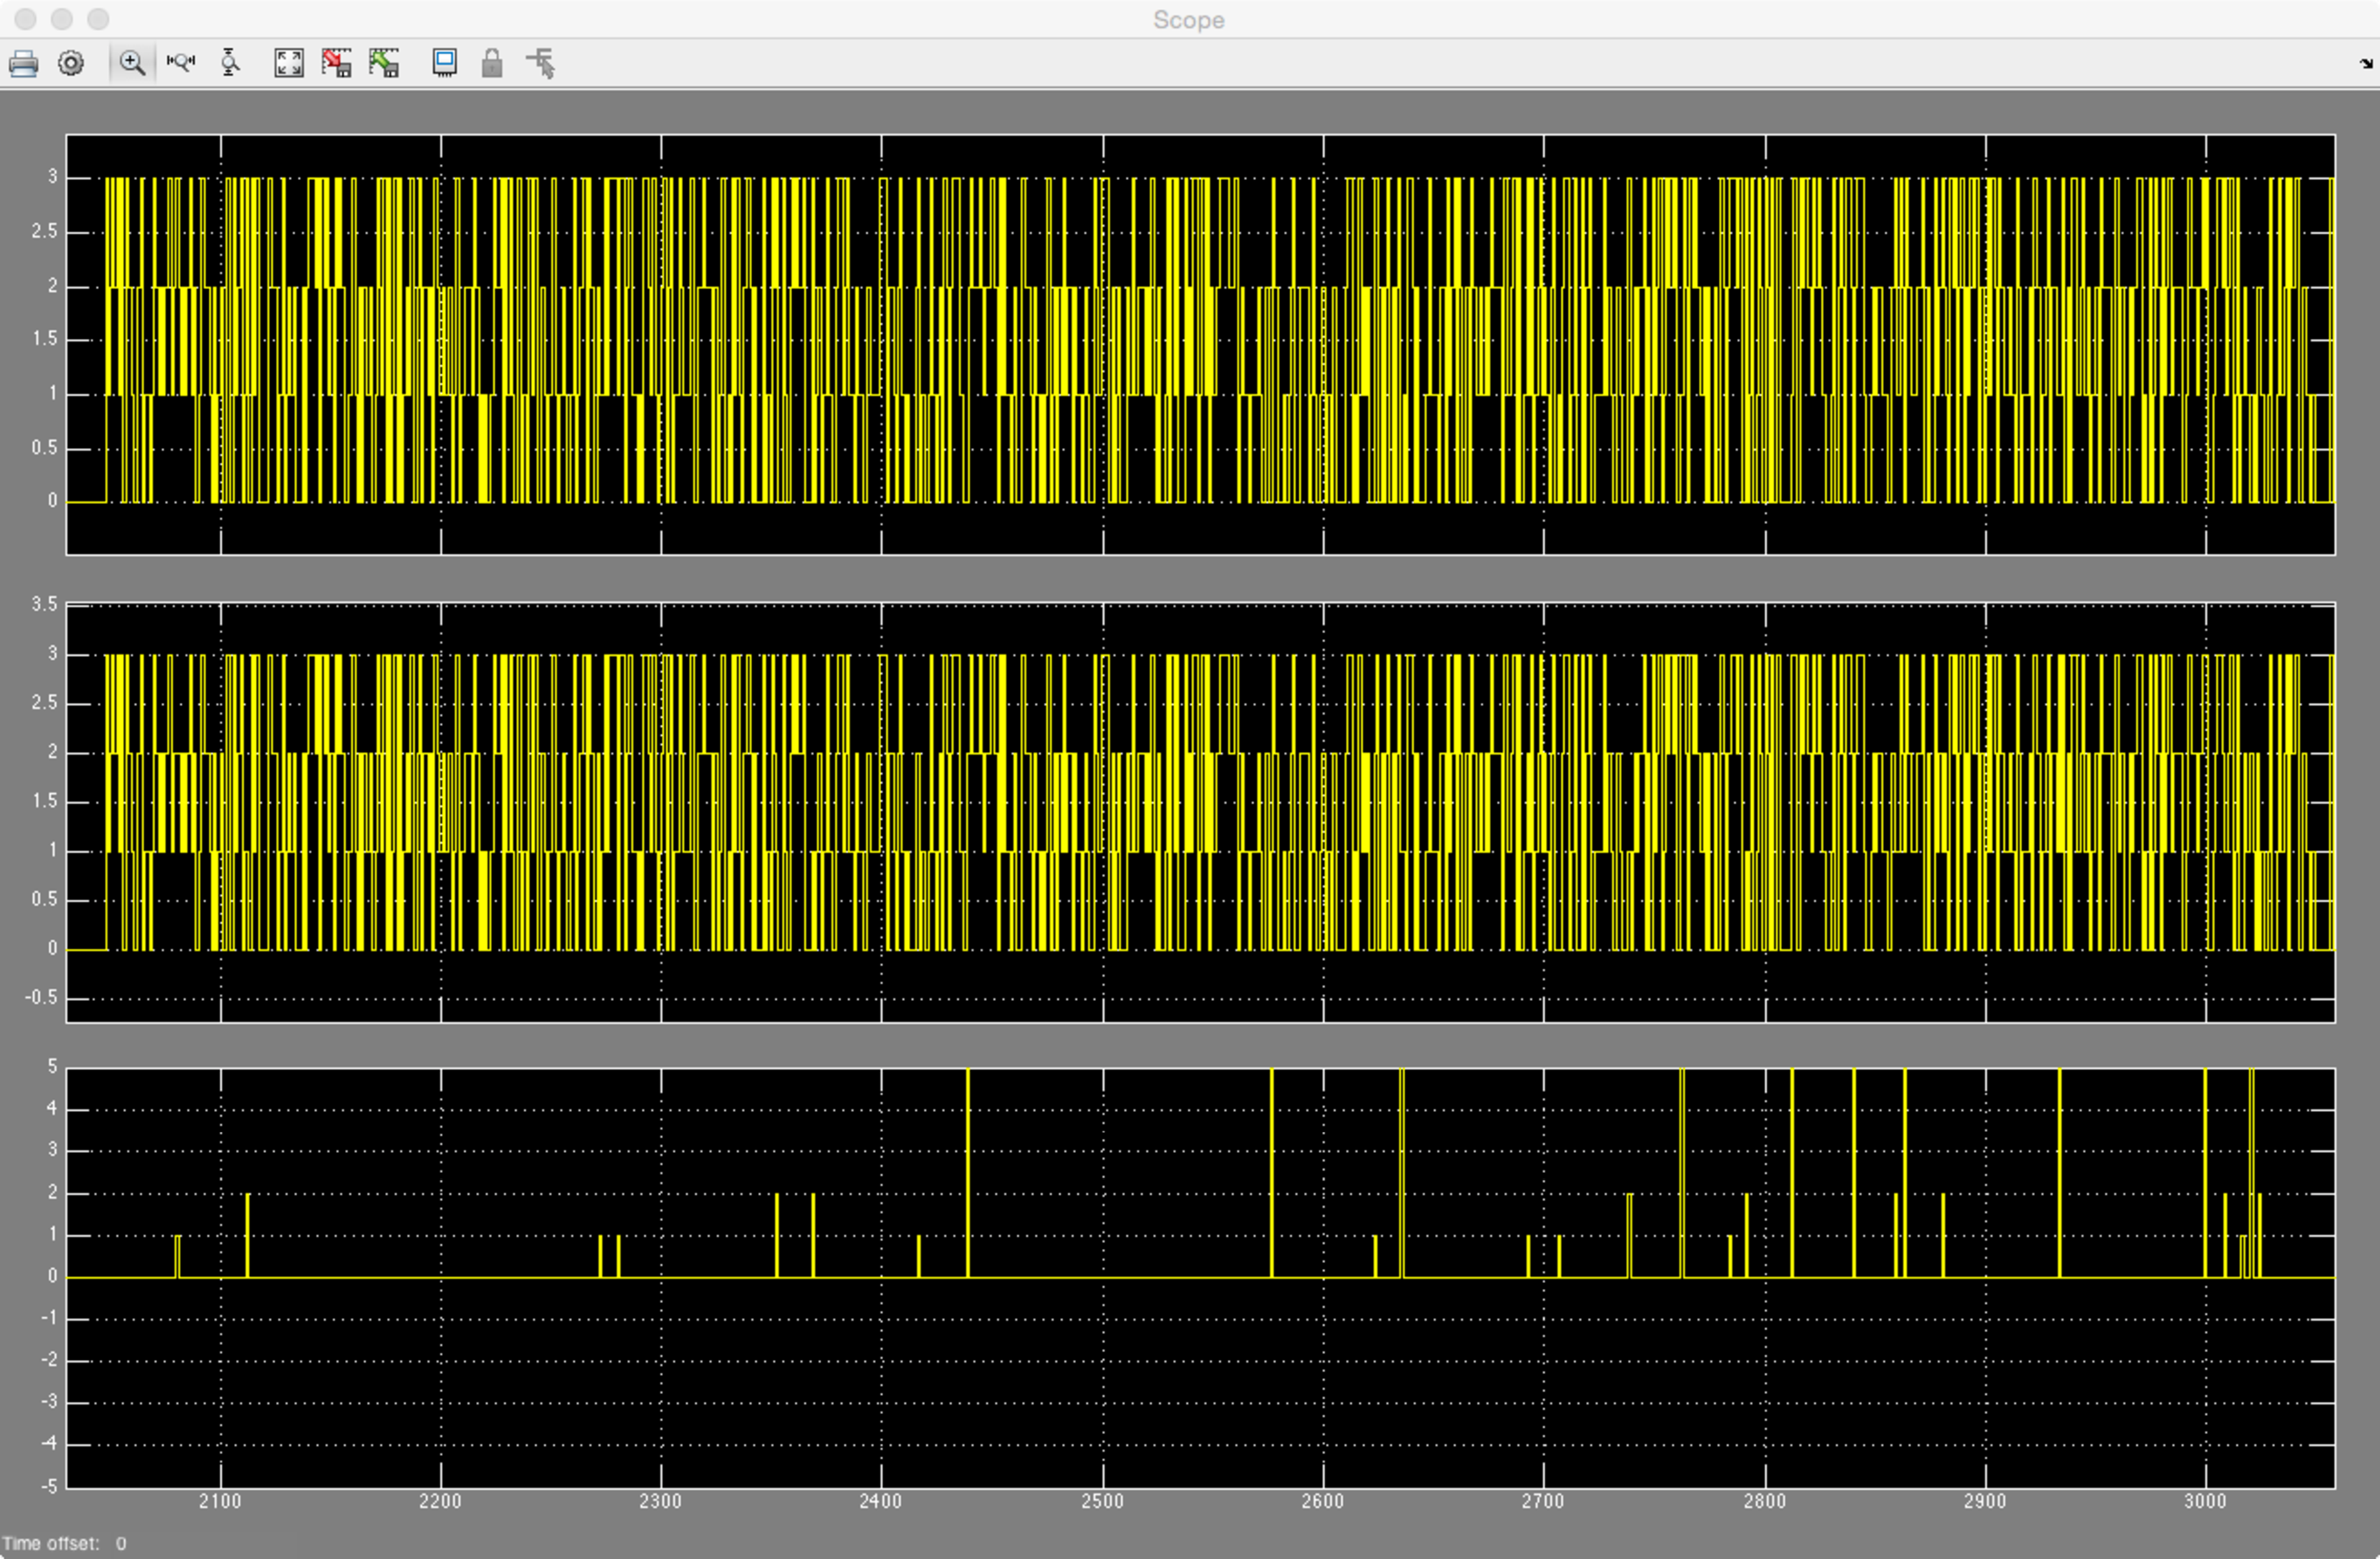
\includegraphics[width=5.5in]{images/ofdm_1024a_scope}
\caption{The first two plots shows signal outputs from two different \gls{fft} paths in \texttt{hdlcoder\_ofdm\_fft\_eml\_1024a}. The third scope plots the difference between these two outputs.}
\label{fig:ofdm_1024a_scope}
\end{figure}
 
The third scope channel is feed from subtractor that compares the two parallel receiver constructs (see Figure \ref{fig:ofdm_1024a_scope}). We did something like this in earlier labs, to provide convenient visual verification that two data streams matched. \textbf{Where is the 2\% error coming from?} Hint: try scoping the respective outputs of the Behavioral\gls{fft} and \gls{fft} HDL Optimized blocks -- if the \gls{fft}s match, then what is causing the disparity?
 
Click on \texttt{Analysis} at the top of your screen, then \texttt{Fixed Point Tool}, then make sure \texttt{hdlcoder\_ofdm\_fft\_eml\_1024a} is selected and change \texttt{Data type override:} to \texttt{[Floating Point] Double [precision]}. What happens to the bit error rate? What is likely going on here?

Important note: Since the hardware-optimized \gls{fft} generates results in bit-reversed order, we have set the block \gls{fft} to do the same. Thus, we compare the (bit-reversed) results from the two receivers, instead of comparing one receiver's output against the original data sequence that was transmitted. We need to add a bit reversal block to the design to do a proper TX-RX bit error rate comparison, but for the moment take the block \gls{fft} as your golden standard.
 
Now lump the \texttt{\gls{fft} HDL Optimized}, \texttt{458-clock delay}, and \texttt{OFDM Receiver Symbol Detection} blocks into a single subsystem (a series of left clicks, one per block, with Shift held down will do nicely), right click on it, and start HDL advisor.
 
Run the resulting Verilog code through Vivado and report projected FPGA resource usage. Do not worry yet about putting this into a Xillybus environment.
 
Now open \texttt{hdlcoder\_ofdm\_fft\_eml\_1024b.slx}. This is similar, except that we are now checking true symbol error rate of recovered data versus originally transmitted data. How were we able to do this, given that the two \gls{fft}s both output bit-reversed data? Also, why are the two error/difference traces on the scope so different? One runs as expected between -3 and +3, but the other has huge spikes of about 255.
 
Describe the two data sources, and try each one in turn by clicking on the \texttt{Manual Switch}. Feel free to invent your own data source generator and to swap it in.  

Important points from this lab:
 
\begin{enumerate}
\item Simplified 1024-point OFDM system with data on every channel.
\item AWGN channel simulation available -- will inject Gaussian noise at a user-selected SNR.
\item Quantization -- we chose 12-bit precision for the receivers' input -- was this enough? What is our practical upper limit of bits? 
\item Bit reversal -- the data emerge from the receiver in bit-reverse order, but we can compensate if we tell the transmitter its incoming data are also in bit-reverse order.
\end{enumerate}

\section{Part II: High Level Synthesis}
The major portion of the OFDM receiver is a 1024-point \gls{fft}. The \gls{fft} is a more efficient version of the Discrete Fourier Transform (DFT). The \gls{fft} utilizes symmetry in the DFT coefficients to provide a recursive implementation that reduces the runtime from O(N2) to O(N log N) where N is the number of samples in the input signal. 

Your tasks for this part of the lab are: 
\begin{enumerate}
\item Implement a working \gls{fft} module that passes the testbench in HLS.
\item Optimize the \gls{fft} module (create and explore multiple architectures) 
\item Implement and optimize the QPSK decoder.
\item Integrate the \gls{fft} and decoder into a complete OFDM receiver.
\end{enumerate}

\subsection{Materials}

You are largely responsible for generating the testbenches for this project. This can be done by extracted data from the provided Simulink file. We do however provide you with testbenches for the \gls{fft}. This is the major part of the receiver.

You are given a zip file with three folders \texttt{0\_Initial}, \texttt{1\_Subcomponents}, and \texttt{2\_Skeleton\_Restructured}.  Folder \texttt{0\_Initial} contains the files corresponding to the ``software'' version of the \gls{fft}. Folder \texttt{2\_Skeleton\_Restructured} provides a framework for a more optimized \gls{fft} implementation. And folder \texttt{1\_Subcomponents} has a number of subfolders that allow you to create projects for individual functions that you will develop over the project. This is largely for your convenience for testing and development. All of the code developed here will eventually be placed in to \texttt{0\_Initial} and \texttt{2\_Skeleton\_Restructured}.
The structure of each of these folders is largely the same.
\begin{itemize}
\item \texttt{*.cpp}: The place where you write your synthesizable code.
\item \texttt{*.h} header file with various definitions that may be useful for developing your code.
\item \texttt{*\_test.cpp}: Testbench
\item \texttt{out.gold.dat}: ``Golden'' output. The testbench (\texttt{*\_test.cpp}) generates a sample input and calls the corresponding function in \texttt{*.cpp} with that sample input. This output of the function is compared to the expected output. This will indicate PASS or FAIL. If it fails, then the code in \texttt{*.cpp} is incorrect.
\item \texttt{script.tcl} and \texttt{directive.tcl}: These allow you to easily create a project. To do this, open the \VHLS Command Prompt tool (\texttt{Start} $\rightarrow$ \texttt{Xilinx Design Tools} $\rightarrow$ \texttt{Vivado HLS} $\rightarrow$ \texttt{Vivado HLS Command Prompt}) and go to the directory where source files and script files reside by using \texttt{cd} command. Then type \texttt{vivado\_hls script.tcl}. This will create a HLS project automatically, so you do not have to add source files, set the top function, select the target device, etc. This will create a folder called \texttt{hls} in that directory with the project. It will also synthesize the project.
\item There is a \texttt{README.txt} which contains a link to the project instructions (this file). \note{probably remove this.}
\end{itemize}

\subsection{Goals}
Part II of the project is divided into stages. The first part of the project is to perform the bit reversal of the input data. Then you optimize a ``software'' version of the code which we have given you (minus the bit reversal portion). After that, you will create a more hardware friendly \gls{fft} architecture. We have provided a testbenches for the individual functions in addition to the testbenches for the overall \gls{fft}. Finally, you must design and implement at QPSK decoder, and integrate it with the \gls{fft} to complete the receiver.

While the major goal of this project is create a functional core, you will also perform optimizations on the code. You should modify the code to create a number of different architectures that tradeoff between performance and area. You will create a report describing how you generated these different architectures (code restructuring, pragmas utilized, etc.). For each architecture you should provide its results including the resource utilization (BRAMs, DSP48, LUT, FF), and performance in terms of throughput (number of \gls{fft} operations/second), latency, clock cycles, clock frequency (which is fixed to 10 ns).

\subsection{\gls{fft} Bit Reversal}
The first step in most optimized \gls{fft} implementation is to reorder the input data by performing ``bit reversed'' swapping. This allows for in-place computation of the \gls{fft}, i.e., the resulting ``frequency domain'' data (as well as the intermediate results) can be stored into the same locations as the input ``time domain'' data. In addition, the output frequency domain data will be in the ``correct order'' at the end of the computation.

An example of the bit reversed data for an 8 point \gls{fft} is shown in Table \ref{tab:bit_reverse}.
\begin{table}[htbp]
\caption{The data for an \gls{fft} must be swapped in a ``bit reverse'' manner. The table shows the decimal value, corresponding binary value, and the reversed binary and decimal values for an 8-point \gls{fft}. }
\begin{center}
\begin{tabular}{|c|c|c|c|}
\hline
Input & Input  & Reversed  & Reversed  \\
Decimal & Binary & Binary & Decimal \\
Address & Address & Address & Address \\
\hline
0 & 000 & 000 & 0 \\
\hline
1	& 001 &	100	& 4 \\
\hline
2	& 010	& 010	& 2 \\
\hline
3	& 011	& 110	& 6 \\ 
\hline
4	& 100	& 001	& 1 \\
\hline
5	& 101	& 101	& 5 \\
\hline
6	& 110	& 011	& 3 \\
\hline
7	& 111	& 111	& 7 \\
\hline
\end{tabular}
\end{center}
\label{tab:bit_reverse}
\end{table}%

In other words, the input data that was initially stored in the array at location 1 is stored in location 4 after the bit reversal is completed. The input data stored in the array at location 4 will be put in array location 1. The input data stored in locations 0, 2, 5 and 7 stay in those locations. Note that this is only true for an 8 point \gls{fft}. Other sizes of \gls{fft} will have different reordering of the data though it is still based on the bit reversed pattern. For example, in a 16 point \gls{fft}, the input data stored in location 1 (binary 0001) will be relocated into location 8 (binary 1000).

You should create an architecture that, efficiently as possible, transforms the input data into a bit reversed order. Note that there are many ``software'' implementations of this that will not effectively map to ``hardware''. While the first goal is to get a working function, you should also consider the performance of the architecture.

We have given you a set of files that allows you to develop and test this bit reversal code in isolation. This includes a simple testbench that exercises this function directly. You should develop and optimized your bit reversed code here. You will later copy this code into the \gls{fft} code.

This code is in subfolder \texttt{1\_bit\_reverse} in the folder \texttt{1\_Subcomponents}. You should develop your code here to insure that it matches the expected result. Note that this testbench is exercising only one input/output result. In other words, even if it passes this, it may not pass all results. Feel free to add additional testbenches to insure your code is correct.

The bit reverse function has the following prototype: \texttt{void bit\_reverse(DTYPE X\_R[SIZE], DTYPE X\_I[SIZE])}

You should perform the swapping ``in place'' on the data in both of the real and imaginary portions of the data. That is the input data in both \texttt{X\_R} and \texttt{X\_I} will be reordered when the function completes.

Your report should describe your code and its performance and area results. Focus on how you modified your code in order to make it more ``hardware friendly''.

Hint: Logical operations map well to hardware. Calculating the indices of the arrays that should be swapped can be done with logical operations. 

\subsection{Optimizing the ``Software'' Version of the \gls{fft}}
The next portion of this lab performs optimization on a typical software implementation of the \gls{fft}. You are given typical three nested loop implementation of the \gls{fft} in the folder \texttt{0\_Initial}. First, you should understand in detail what this code is doing. It is worth spending time on this now as you will have to rewrite the \gls{fft} in a more hardware friendly manner in the next steps. You can reuse some of this code in those steps.

You should optimize this code as much as possible and detail these optimizations and their performance area results in your report. The results of the code will be poor; it will likely have greater than 250 million cycles. The throughput here is likely much worse than running this in software on a microprocessor. This often happens when we put the initial software versions of an application into a high level synthesis tool. And it should not be all that surprising. The code is optimized to run quickly in software, which runs largely in a sequential model of computation. The code must typically be carefully optimized with the final hardware architecture in mind to get good results. This involves exploiting parallelism and pipelining.

You will also notice that the first loop has function calls to sine and cosine. This code will synthesize quickly with these function calls. However, you may wish to replace these function calls (which will synthesize into CORDIC cores), into table lookups. We have provided two tables in the \texttt{.h} file, \texttt{W\_real} and \texttt{W\_imag} which contain the precomputed twiddle factors for our 1024 \gls{fft}, i.e., \texttt{W\_real[i] = cos(2.0*pi*i/SIZE)} and \texttt{W\_imag[i] = sin(2.0*pi*i/SIZE)} where $i = [0,512)$.

Some potential optimizations include:
\begin{itemize}
\item Using the \texttt{W\_real} and \texttt{W\_imag} tables.
\item Pipelining
\item Loop unrolling
\item Memory partitioning
\end{itemize}

In the report, you should discuss the performance and area numbers of the various optimizations that you apply. This must describe the effect of these optimizations on the architecture, and not just state the optimization that you used.

\subsection{Hardware Friendly \gls{fft} Implementation}

A good architecture will selectively expose and take advantage of parallelism, and allow for pipelining. Your final \gls{fft} architecture will restructure the code such that each stage is computed in a separate function or module. There will be one module for bit reversal that you have already developed, and then $\log N$ stages (10 in our case) for the butterfly computations corresponding to the 2-point, 4-point, 8-point, 16-point, \dots \gls{fft} stages.

The skeleton code for this final \gls{fft} implementation can be found in the \texttt{2\_Skeleton\_Restructured} folder. This creates code connects a number of functions in a staged fashion with arrays acting as buffers between the stages. Figure \ref{fig:staged_fft} provides a graphical depiction of this process.

\begin{figure}
\centering
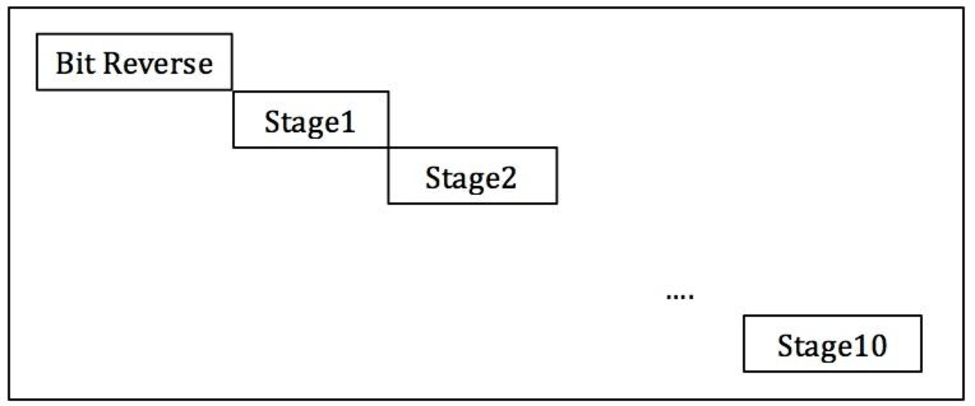
\includegraphics[width=5.5in]{images/staged_fft}
\caption{A staged implementation of a 1024 \gls{fft}. Bit reversal is followed by 10 stages of butterfly computations. This architecture is capable of pipeline both within the stages and across the stages.}
\label{fig:staged_fft}
\end{figure}

The first step in this process is to create code that computes the first and last stages of the \gls{fft}. The hope is that this will allow you to get a better understanding of exactly how memory accesses and the butterfly computations are performed in a general case. You can develop these two functions \texttt{fft\_stage\_first} and \texttt{fft\_stage\_last} in isolation. They both have subfolders in the \texttt{1\_Subcomponents} folder. Once these are working correctly, you can copy and paste the code directly in the same functions in the \texttt{2\_Skeleton\_Restructured} project.

The next task is to create code that can implement ``generic'' function, i.e., one that can compute any stage of the \gls{fft}. This is the function \texttt{fft\_stages} which also has its own project in the \texttt{1\_Subcomponents} folder. Note that this function prototype is similar to \texttt{fft\_stage\_first} and \texttt{fft\_stage\_last} with one major difference: it has a stage argument. This code will used to implement stages 2 through 9 in the \texttt{2\_Skeleton\_Restructured} project.

Hints:
\begin{enumerate}
\item These stages are performing the same calculation as one iteration of the outer for loop in the \texttt{0\_Initial} project.
\item The major difference between the stages is what data elements you are performing the butterfly functions on, i.e., in what order do you pull data from \texttt{X\_R} and \texttt{X\_I}.
\item Test each of the functions in isolation with the provided projects. Make sure that the code compiles and passes the testbench before attempting any optimizations.
\end{enumerate}

Once you have a correctly functioning set of functions, you should copy and paste them in the \texttt{2\_Skeleton\_Restructured} project and make sure that it passes the testbench. Since our testbenches perform one check, which is far from comprehensive, it is possible, though hopefully unlikely, that you have some error that the \texttt{2\_Skeleton\_Restructured} testbench exposes and was not exercised in the individual testbench. If your code passes the \texttt{2\_Skeleton\_Restructured} project you can assume it is correct (though again since it is only one test, it may be wrong; you should perform significantly more testing if you want this to be anywhere close to production quality).

Now on to the final part of the project, optimizing of this restructured code. You should perform the typical tricks here: pipelining, memory partitioning, unrolling, etc. Some of these may not make sense depending on how you wrote your code. This final architecture should be orders of magnitude better than the \texttt{0\_Initial} project. Highly optimized \gls{fft} architectures can easily have less than 10000 cycles.

You should describe in your report the baseline results and the effects of any optimizations that you performed. By this point, you should be starting to understand what optimizations will work and which will not work, and most importantly why. Describe these insights in your report.

\subsection{QPSK Decoder}
The decoder takes the 1024 I/Q outputs from the \gls{fft} and decodes them into the corresponding binary data. Essentially you have to reverse the encoding that was done in the transmitter. The encoder went from 0 and 1 to -1 and 1. Because you have a perfect channel, the output of your \gls{fft} will be -1 and 1. You must make those into 0 and 1. You can look at the Simulink file to determine the exact encoding. It used a Gray code, and the constellation taken directly from the Simulink file is shown below.

\begin{figure}
\centering
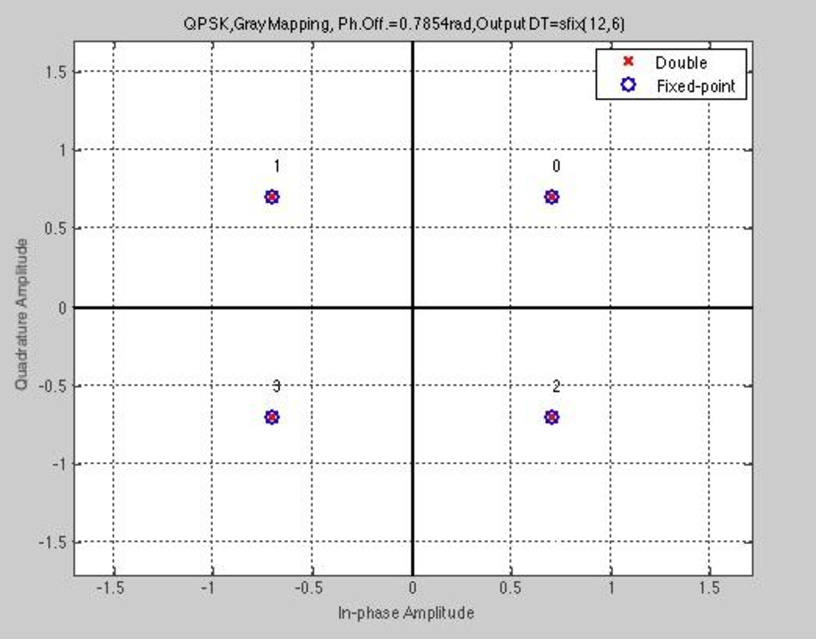
\includegraphics[width=5.5in]{images/qpsk_fft}
\caption{A QPSK constellation using a Gray mapping for translating into the I and Q values.}
\label{fig:qpsk_fft}
\end{figure}

The output of your encoder should be the exact data that was given to the OFDM receiver in the Simulink file. You can create your testbench to reflect this.

\subsection{Receiver Integration}
You should connect the \gls{fft} and the QPSK decoder together to form the complete OFDM receiver. The input to the receiver is the data from the channel. The output of the receiver should match the transmitted data.

\subsection{Optimization Hints and Report Guidelines}

\begin{itemize}
\item You should use a clock period of 10 ns. While varying the clock period can drastically change the results, this is not a focus of this project. Though feel free to modify this and observe the changes. 
\item The output of the various architectures that you generate must match the golden output. We have broken down the project into subcomponents to allow you to develop and test them individually. You would be wise to do it in such a manner.
\item You should not change the data types as given to you. You do not need to perform bitwidth optimization of this project.
\item There are some variable defined in the \texttt{.h} files for you convenience. These include \texttt{SIZE = 1024}, \texttt{SIZE2 = 512}, and \texttt{M = 10} (i.e., $\log$ SIZE). Feel free to use these in your code. They are defined in every \texttt{.h} file across all of the different folders.
\item The major goal of this project is to get fully functional versions of all the code. You should focus more of your time on getting everything to work rather than getting some but not all of the components to work and optimizing them.
\item Your report should describe your code at a high level. Since each of you will likely write different code anyone that reads your report should be able to fully understand what each line of your code does. However, this does not mean that you need to explain each line of code in excruciating detail. It is possible to be succinct and thorough at the same time.
\item The software version has a nested for loop structure that does not allow Vivado HLS to provide an exact number of cycles. The \texttt{tripcount} directive can help with this. You should be able to understand the reported results. For example, while Vivado may give you a best, worst and average case numbers, your algorithm for a fixed size \gls{fft} should be a fixed number of cycles. You should report the exact number of cycles for your throughput numbers. You must describe in your report exactly how you derived your throughput results.
\item You must provide a comparison between the best architecture that you derived using the ``software'' version and the best one using the ``hardware friendly'' framework.
\item It is ok to rewrite the code if it helps you with optimizations. For example, you can change the function interfaces.
\item Your code should be written such that the hardware implementation is optimal. For example, there are many ways to do a bit reversal that are efficient in software but not necessarily efficient in hardware.
\item Comment your code.
\end{itemize}

\section{Part III: Zedboard Demo}
You must implement the entire OFDM receiver on the Zedboard in the programmable logic. You should use Xillybus to transmit data to the receiver, the receiver operates on the data, and you will use Xillybus to get the data off of the programmable logic and back onto the ARM core. You must use Gplot to show that transmitted and the received data. 

You are responsible for extracting the transmitted data from the Simulink testbench. You can use ``To Workspace'' data from any signal in the Simulink file. This will then appear as a variable in the Matlab workspace. There are already several ``To Workspace'' blocks in your Simulink file that you can either use directly or modify to extract the necessary data. You only need to show one ``frame'', i.e., the data from the output of one 1024 \gls{fft}.

We provided the general framework for Gplot, Xillybus, etc. in previous labs. You should use that to create this demo. We will not be providing you with anything more than what was given in previous labs. You should provide a plot similar to Figure \ref{fig:ofdm_zedboard} in your report to prove your design is working.  Please plot the entire 1024-point output. Please also plot a zoomed-in version of the output. We would like to see the ``0 1 2 3 0 1 2 3 0 1 2 3 \dots'' sequence clearly.

\begin{figure}
\centering
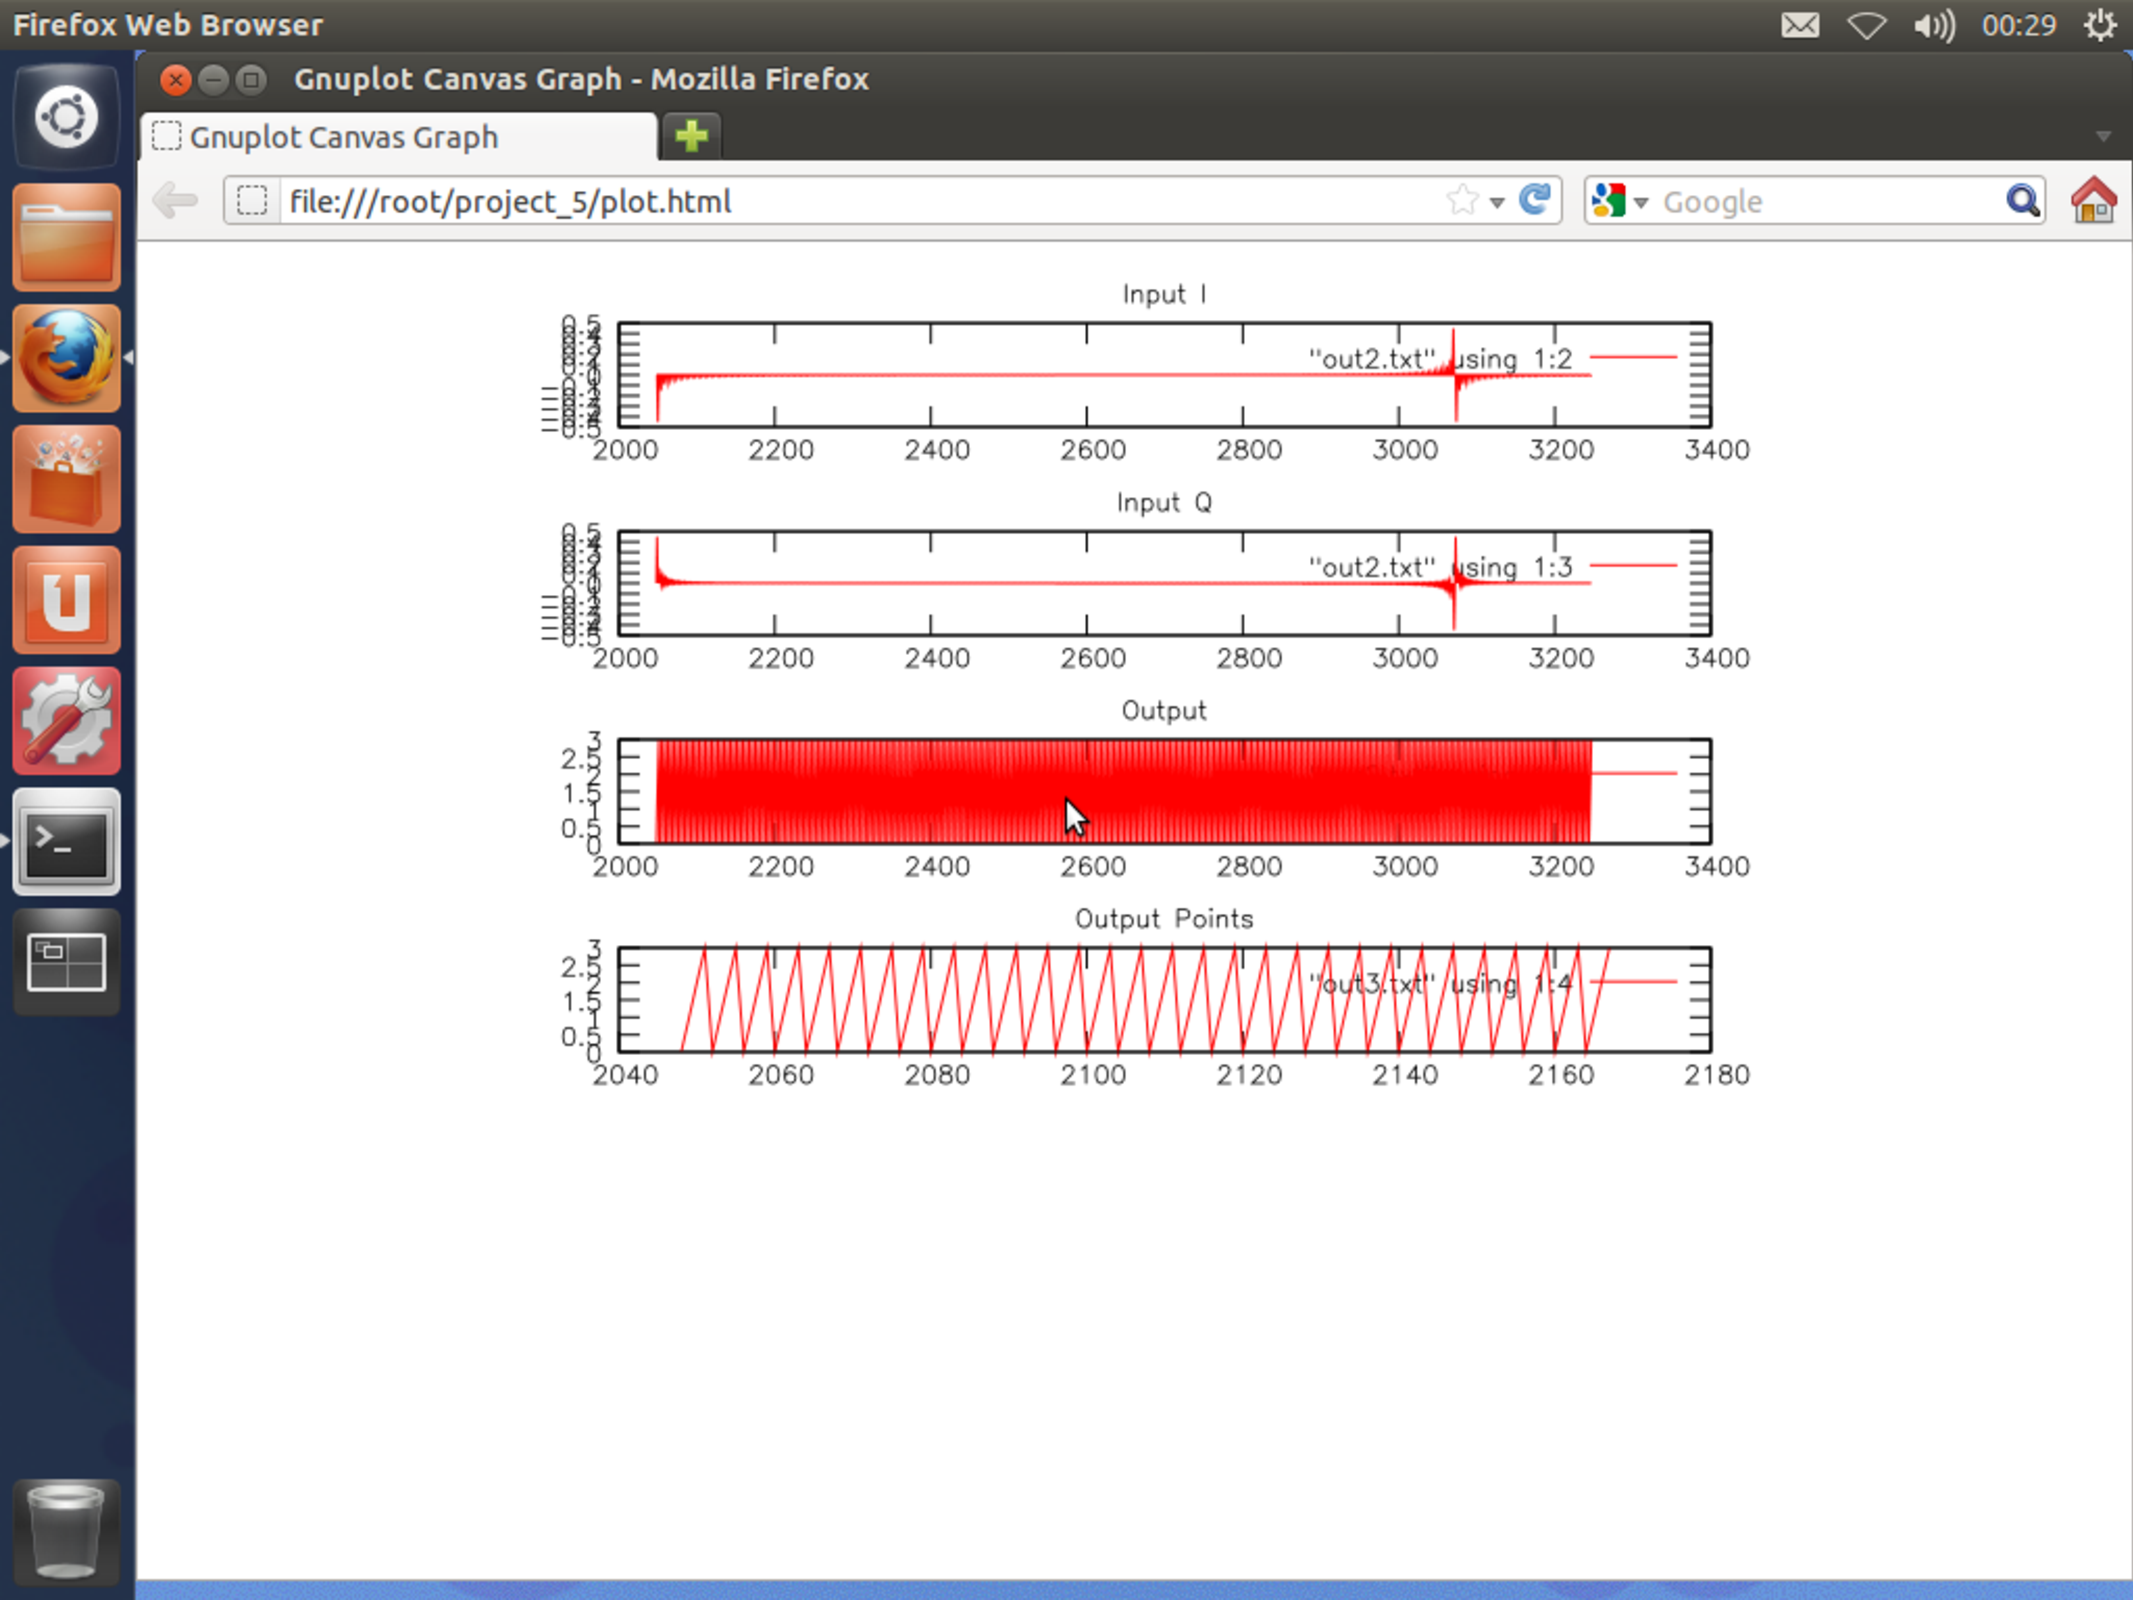
\includegraphics[width=6in]{images/ofdm_zedboard}
\caption{An example plot showing the input and output values to the simple OFDM receiver.}
\label{fig:ofdm_zedboard}
\end{figure}
